\chapter{Materials and methods}
In this chapter, we describe the steps performed in the project.
Firstly, we provide a general overview of the pipeline. 
Next, we continue with the presentation of data which were available to us and which we used.
Then we describe in detail how we processed them to the form suitable as input for our neural network.
Finally, we show how we designed our neural network in detail and how we tested the performance of our designs.

\section{The pipeline}
We recorded each step of our analysis in the primary analysis file named Snakefile.
This file is executable using Snakemake workflow management system\cite{koster2012snakemake}.
The main reason to use this workflow management system was to make our analysis reproducible.
Snakemake also increases the readability of the procedure and make orientation in the scripts more straightforward.
Snakefile consists of rules, which define necessary input, output and the code needed for producing the output from the input.
These rules can be visualised as a directed acyclic graph symbolising the order of execution.
In Figure \ref{fig:dag}, we provide a simplified graph containing all the rules and their dependencies.

\begin{figure}
    \centering
    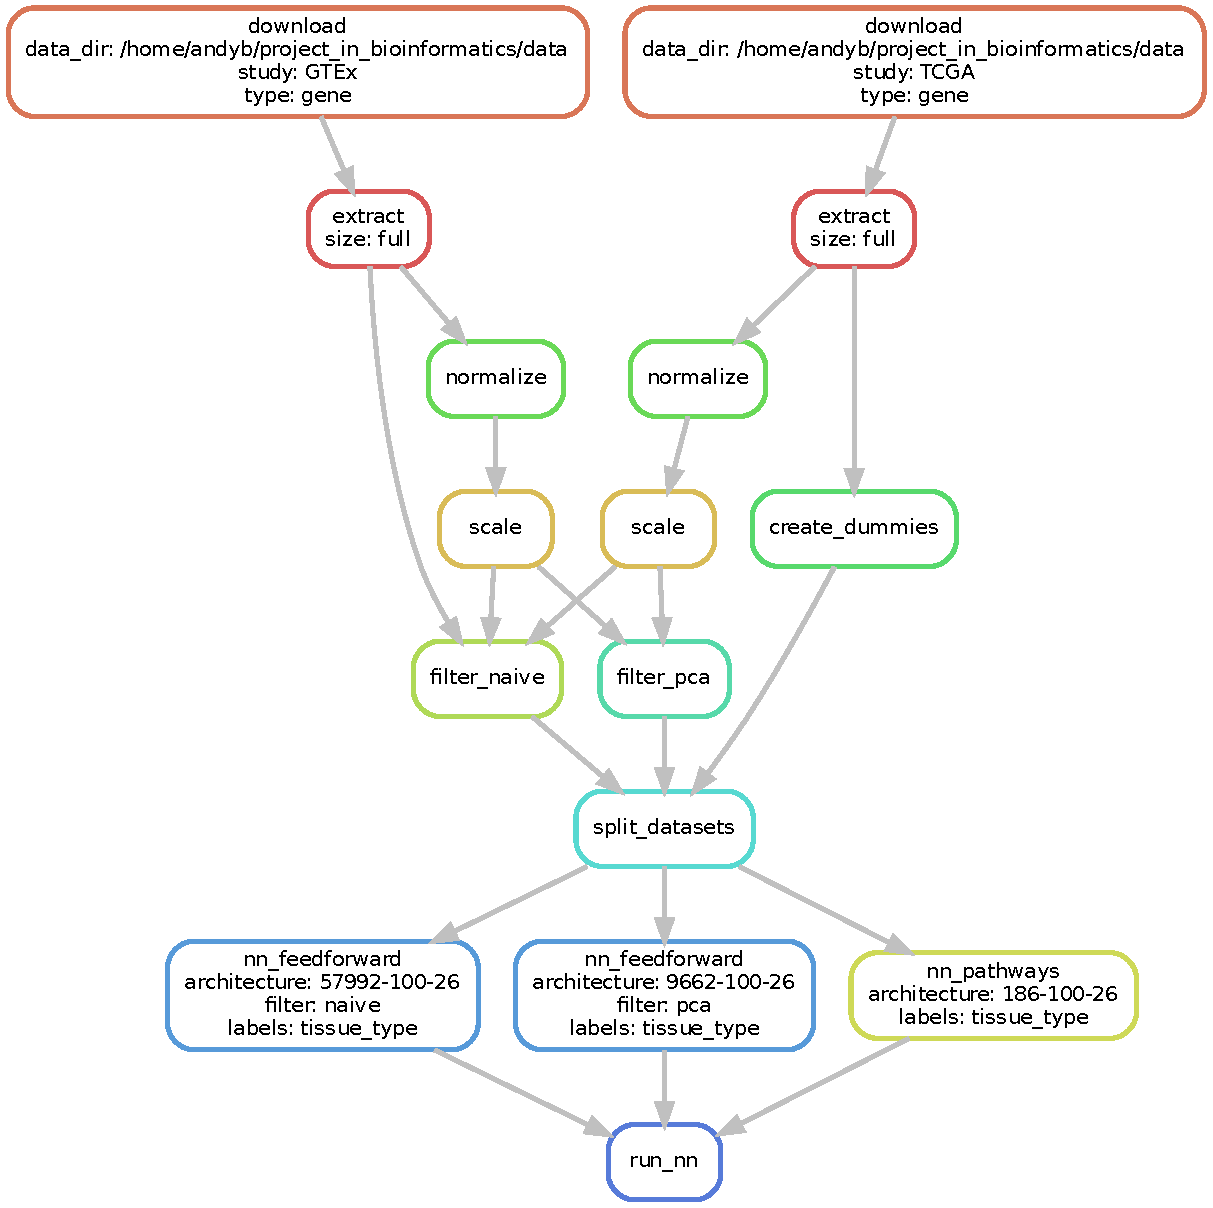
\includegraphics[width=\linewidth]{images/dag.pdf}
    \caption[Pipeline overview]{Pipeline overview: Nodes represent the executed rules, arrows represent the flow of information. This example used fewer parameters in comparison with the real run.}
    \label{fig:dag}
\end{figure}

\newpage
\section{Data available}
The main data which we worked with consisted of RNA-seq gene counts.
RNA sequencing has become a standard in studying a gene expression mainly due to its ability to detect transcriptional activity even without previously defined gene sequence\cite{nellore2016rail}.
A common use of this method is to determine expression level across the samples and then use this information to identify the patterns associated with the outcome of interest.
In our project, we used expression data from two distinct sources, The Genotype-Tissue Expression project (GTEx)\cite{lonsdale2013genotype} and The Cancer Genome Atlas (TCGA)\cite{tcga}.

\subsection{TCGA}
The Cancer Genome Atlas Program is a joint effort between the National Cancer Institute and the National Human Genome Research Institute.
Since the year 2006, they provide access to one of the most comprehensive datasets of multiple types of cancer.
TCGA generated over 2.5 petabytes of genomic, epigenomic, transcriptomic and proteomic data to improve our abilities to diagnose, treat a prevent cancer.
These data are publicly available to researchers all around the world.

\subsection{GTEx}
The Genotype-Tissue Expression project was established to create a data resource to study genetic variation, the regulation of gene expression and other molecular phenotypes.
The dataset contains expression data from multiple reference tissue types and is freely available online.

\subsection{KEGG pathways}
Another database used in our analysis is the Kyoto Encyclopedia of Genes and Genomes (KEGG) \cite{kanehisa2000kegg}.
This database contains information useful for systematic analysis of gene function and linking genomic information with higher order functional information.
The higher order functional information is characterized as cellular processes, such as metabolism, membrane transport, signal transduction and cell cycle.
In the project, we used the information of the gene membership to particular pathways.
\label{subsec:kegg}

\subsection{Downloading}
Downloading of the expression data was done using R package \verb'recount' \cite{collado2017reproducible}.
We created a custom R script for downloading TCGA expression dataset and GTEx expression dataset.
The downloaded expression data were stored as \verb'RangedSummarizedExperiment' object in the file with the extension \verb'.Rdata'.
This object is designed to select data of interest from the large dataset.
The outline of the object structure can be found in Figure \ref{fig:sre}.
In the case of expression data, the rows contain genes and all information related to them, and the columns contain samples and their related information.
Unfortunately, because we wanted to perform our analysis mainly using python programming language, we needed to convert the downloaded data to another format.
We decided to convert files to tab separated values since this format is widely accepted structuralized data format.
Therefore, for each dataset, we created one file containing gene expression counts, mirroring the structure of assays part of the \verb'RangedSummarizedExperiment' object and two files containing assignments of our response variables to the sample ids.

\begin{figure}
    \centering
    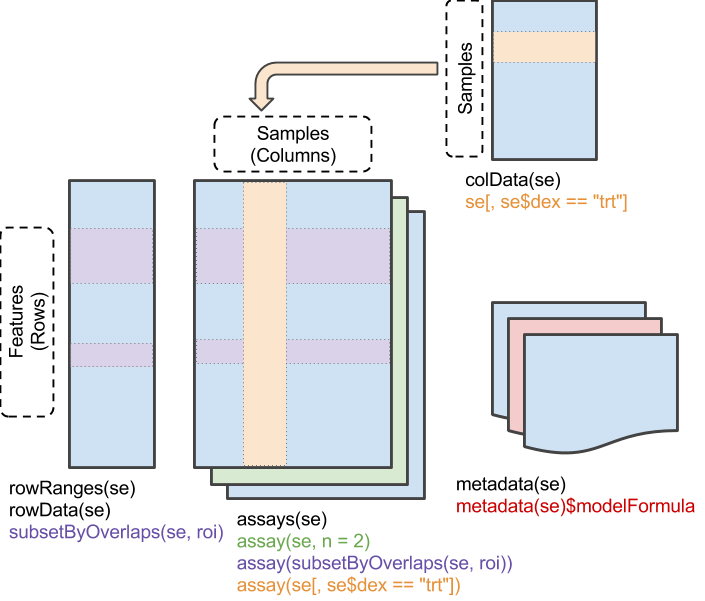
\includegraphics[width=0.8\linewidth]{images/SummarizedExperiment.png}
    \caption[Structure of \texttt{RangedSummarizedExperiment}]{Structure of the \texttt{RangedSummarizedExperiment} object. The rows represent genes, and the columns represent samples. The expression data are stored in the assays part of the object. The structure ensures the correct selection of elements by bounding features to rows and samples to columns.}
    \label{fig:sre}
\end{figure}

\newpage
\section{Data preparation}
Downloaded expression data represented raw counts of the genes.
These raw counts can have multiple problems \cite{robinson2010scaling}.
\begin{enumerate}
    \item Every sample is potentially sequenced to a different depth.
    \item The genes compete for the limited space in the sequencing experiment. Therefore samples with more active genes tend to have lesser expression per gene. 
    \item Genes with longer transcripts have a higher probability of being sequenced.
\end{enumerate}
To mitigate these problems and to ensure high-quality results further down in the pipeline, we performed normalization and scaling of the data.
We also visualized the effects of our normalization and scaling to assess the correctness of our steps.

\subsection{Normalisation}
Because of the different depth in the sequencing experiments, it was necessary to perform normalisation of our data.
The first idea was to divide each expression entry by the median of that particular sample.
This procedure should eliminate the problem with variable depth and potentially the problem with genes competing for limited space in the experiment.  
Unfortunately, in cases with shallow coverage, the median value of the expression was zero, which caused division by zero error in insufficiently covered samples.
Therefore we decided to divide entries by the 75th percentile of a particular sample.
This division had a similar effect as dividing by median, and we overcome the division by zero problems in all samples.
After normalisation with 75th percentile, we also performed a logarithmic transformation of our data.
This procedure helped to reduce the strong left skew of the data and ensured that our data looked more normally distributed.
The effect of this step was visualized in the Figures \ref{fig:expr_dist} and \ref{fig:norm_expr_dist}.

\begin{figure}
    \centering
    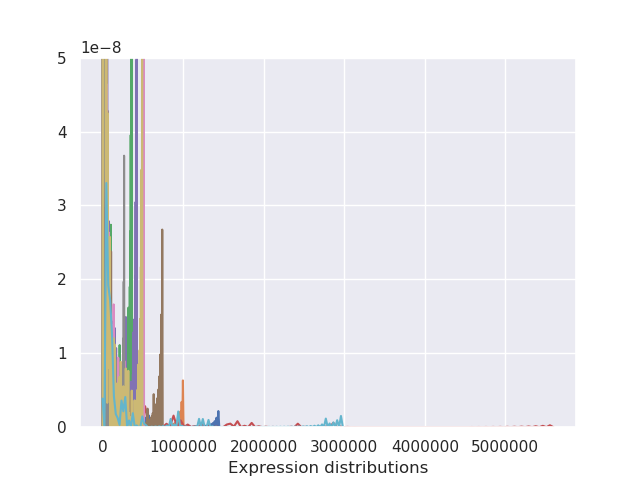
\includegraphics[width=0.8\linewidth]{images/expr_dist.png}
    \caption[Expression before normalization]{Expression distributions of the first 10 samples before the normalization}
    \label{fig:expr_dist}
\end{figure}

\begin{figure}
    \centering
    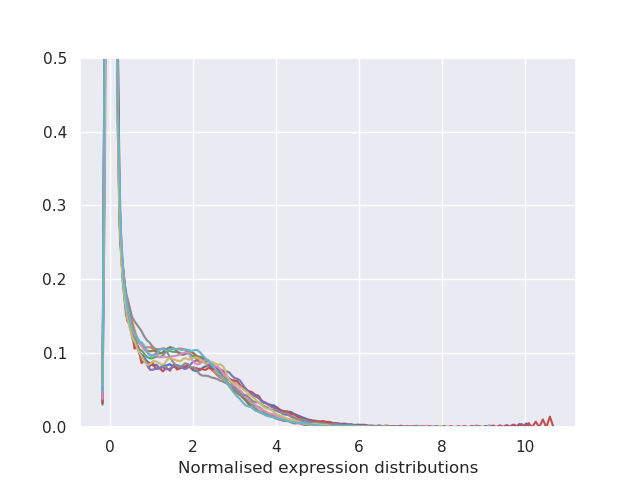
\includegraphics[width=0.8\linewidth]{images/norm_expr_dist.png}
    \caption[Expression after normalization]{Expression distributions of the first 10 samples after the normalization}
    \label{fig:norm_expr_dist}
\end{figure}

\subsection{Scaling}
In the scaling step, we tackled the problem, that longer transcripts tend to have a higher probability of being sequenced.
We decided to solve this issue by adjusting each gene to have mean zero and standard deviation one.
In comparison with the previous step, we performed row-wise standardization instead of column-wise.
Performed standardization was according to the Equation \ref{eq:std}.
The effect of this step was visualized in the Figure \ref{fig:norm_expr_genes} and \ref{fig:scaled_expr_genes}.

\begin{equation}
    x_{ij} = \frac{x_{ij}-\bar{x_{i}}}{sd(x_{i})}
    \label{eq:std}
\end{equation}

\begin{figure}
    \centering
    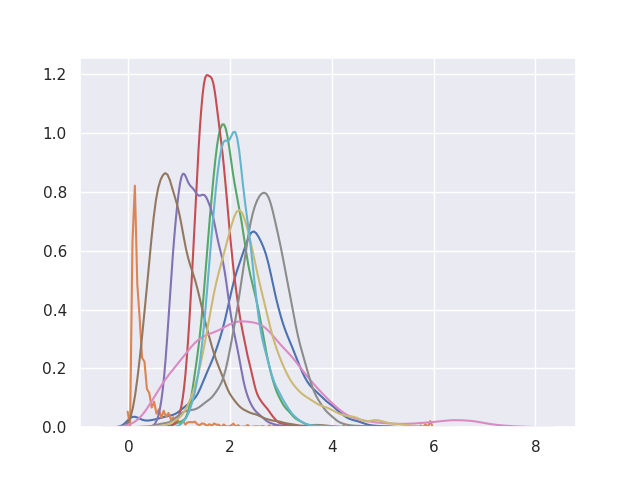
\includegraphics[width=0.8\linewidth]{images/norm_expr_genes.png}
    \caption[Expression before scaling]{Expression distribution of the first 10 genes before the scaling}
    \label{fig:norm_expr_genes}
\end{figure}

\begin{figure}
    \centering
    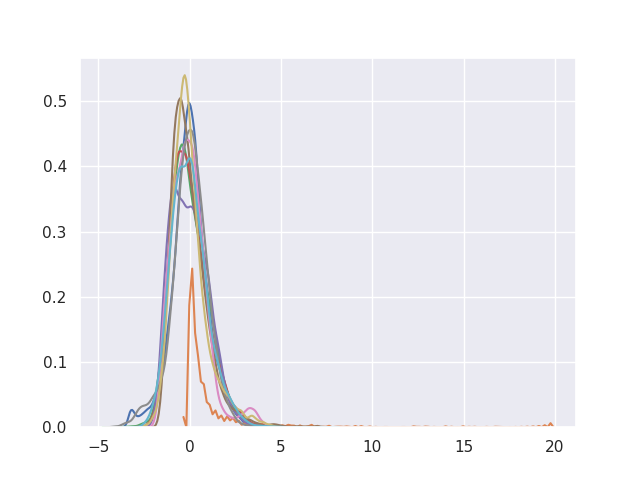
\includegraphics[width=0.8\linewidth]{images/scaled_expr_genes.png}
    \caption[Expression after scaling]{Expression distibution of the first 10 gene after the scaling}
    \label{fig:scaled_expr_genes}
\end{figure}

\newpage
\section{Filtering}
In the filtering step, we tried to select the best predictors for our outcomes.
This step should help the analysis for multiple reasons.
\begin{enumerate}
    \item The number of genes largely exceeds the number of samples. This fact could lead to overfitting and inability to find the model that is general enough to perform well in practice.
    \item There is a considerable probability that some genes are expressed independently of our response variables. We want to remove those genes from the analysis as they introduce noise to our model.
    \item Some gene expressions might be highly correlated. This fact introduces further complications for our model.
\end{enumerate}
To address these issues, we performed feature selection using two different approaches.

\subsection{The variation of within-group means}
The first criterium for good predictor was the variation of within-group means.
The idea was that most non-informative genes tend to have similar values of gene expression in all tissue types.
For this step, we used the GTEx dataset.
We grouped the GTEx data according to their associated tissue type and calculated the mean for each gene in each group.
Afterwards, we calculated the variation of the means for each gene.
The genes in TCGA dataset were then sorted according to the calculated variation in descending order.
The sorted order was then used further in the pipeline, where we chose the first few predictors with the highest variation.

\subsection{Principal component analysis}
Principal component analysis (PCA) is a standard method of dimension reduction for high-dimensional data. 
For $(n\times p)$ matrix, it produces $min(n-1, p)$ principal components.
The principal components are a new set of predictors constructed from the original data in such a way that they are linearly uncorrelated.
In addition, the first principal component explains the most of the variance of the original dataset and each next principal component explains most of the remaining variance under the condition that it is orthogonal to all the previous principal components. 

In our project, we used the GTEx dataset to find the transformation needed to create principal components and then used this transformation on the TCGA dataset.
This transformed dataset was then used further in the pipeline.

\newpage
\section{Dataset splitting}
In this step, we split our dataset to training, validation and testing datasets.
We decided to determine the hyperparameters of our models using the validation set approach.
This approach picks a proportion of observations from our training data, which are then not used in the training of the model.
Multiple models with different parameters are then built, and the testing accuracy of the models is then approximated using the validation set.
The validation set approach has many drawbacks in comparison with cross-validation methods.
\begin{enumerate}
    \item The estimate of test error is highly dependent on the chosen observations used for validation, and it can vary a lot.
    \item Since we are using just a subset of observations for training, this method tends to overestimate the test error.
\end{enumerate}
Despite these drawbacks, we preferred this approach mainly because of the computational intensity of the training of the neural networks, which could render other approaches computationally infeasible. 

There was another challenging problem of the validation set approach when creating the sets by random selection.
This problem was that there was a considerable probability of not sampling some classes for training dataset at all.
That could create a problem of the heavily unbalanced training sample.
We tried to minimize this effect by performing the splitting as follows.
First, we removed all observations with a missing value of the response variable.
Then we grouped remaining observations by tissue type and by cancer stage.
Finally, we selected randomly 20\% observations as testing set, 20\% observation as validation set and the remaining 60\% observations as the training set.
The effects of this procedure is visualized in the Figures \ref{fig:split_tissue}, \ref{fig:split_stages} and \ref{fig:split_all}. 

\begin{figure}
    \centering
    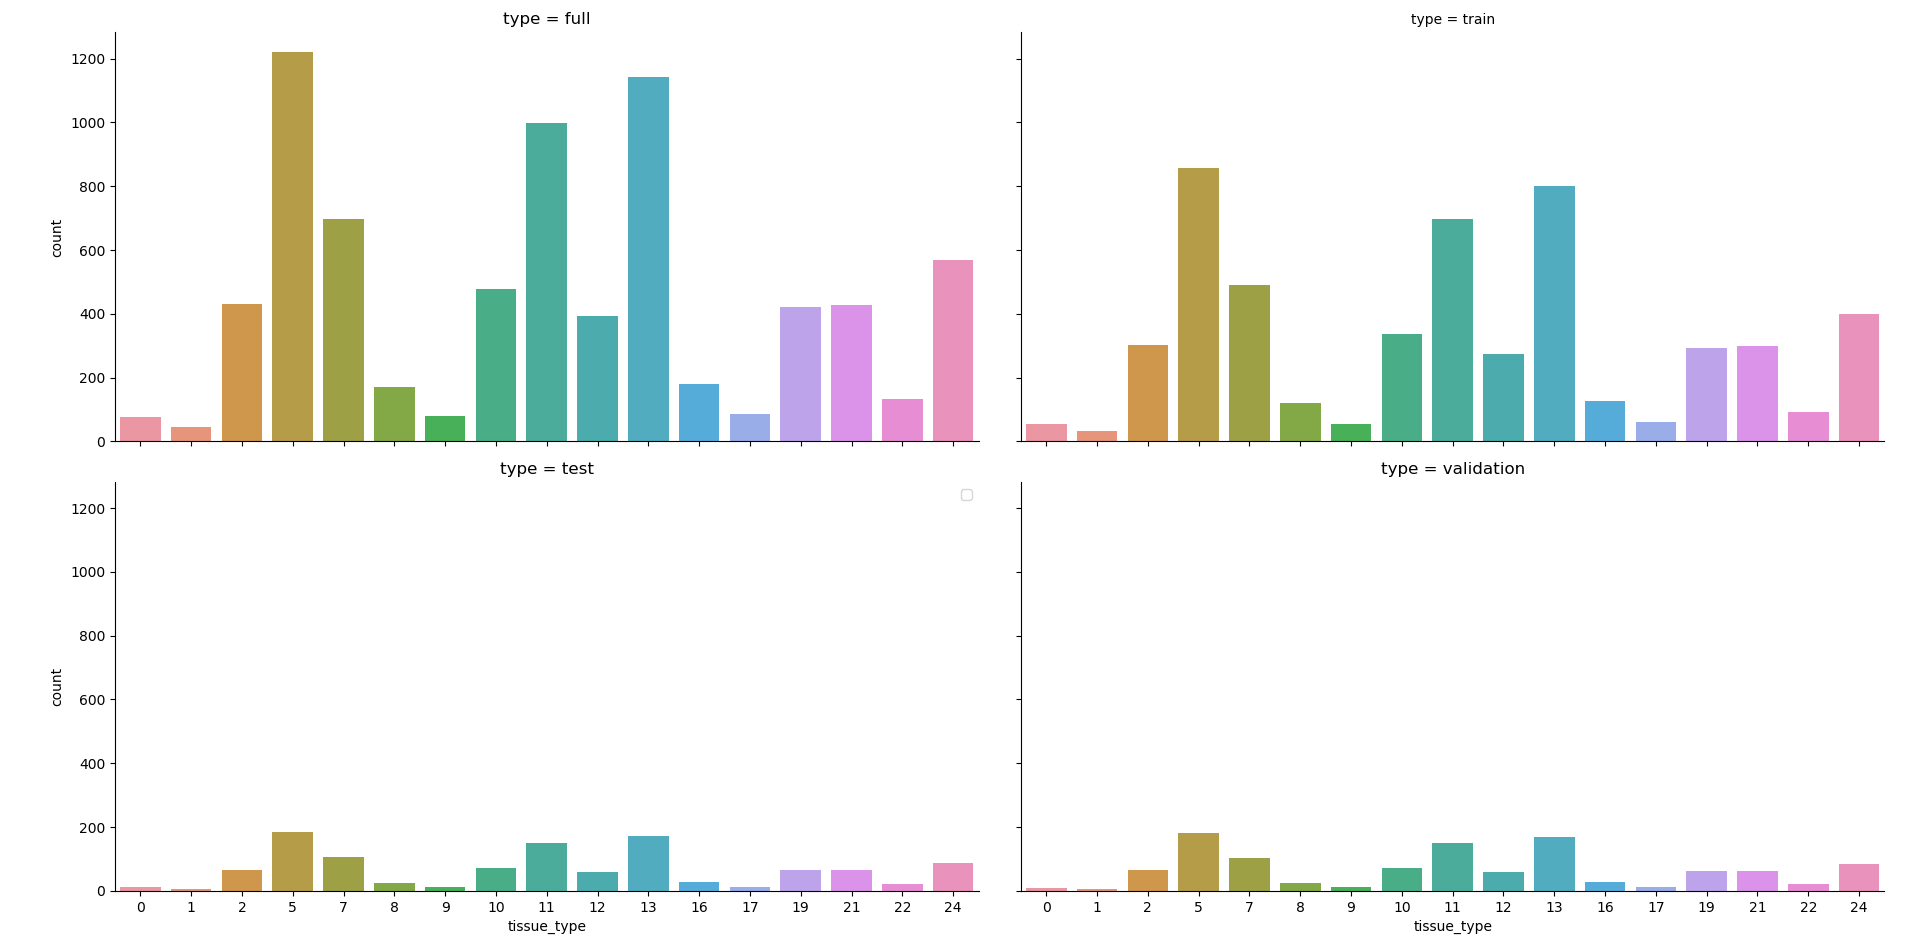
\includegraphics[width=\linewidth]{images/split_tissue.png}
    \caption[Splitting - tissue type]{Splitting of the main dataset to train, validation and test set with respect to tissue type}
    \label{fig:split_tissue}
\end{figure}

\begin{figure}
    \centering
    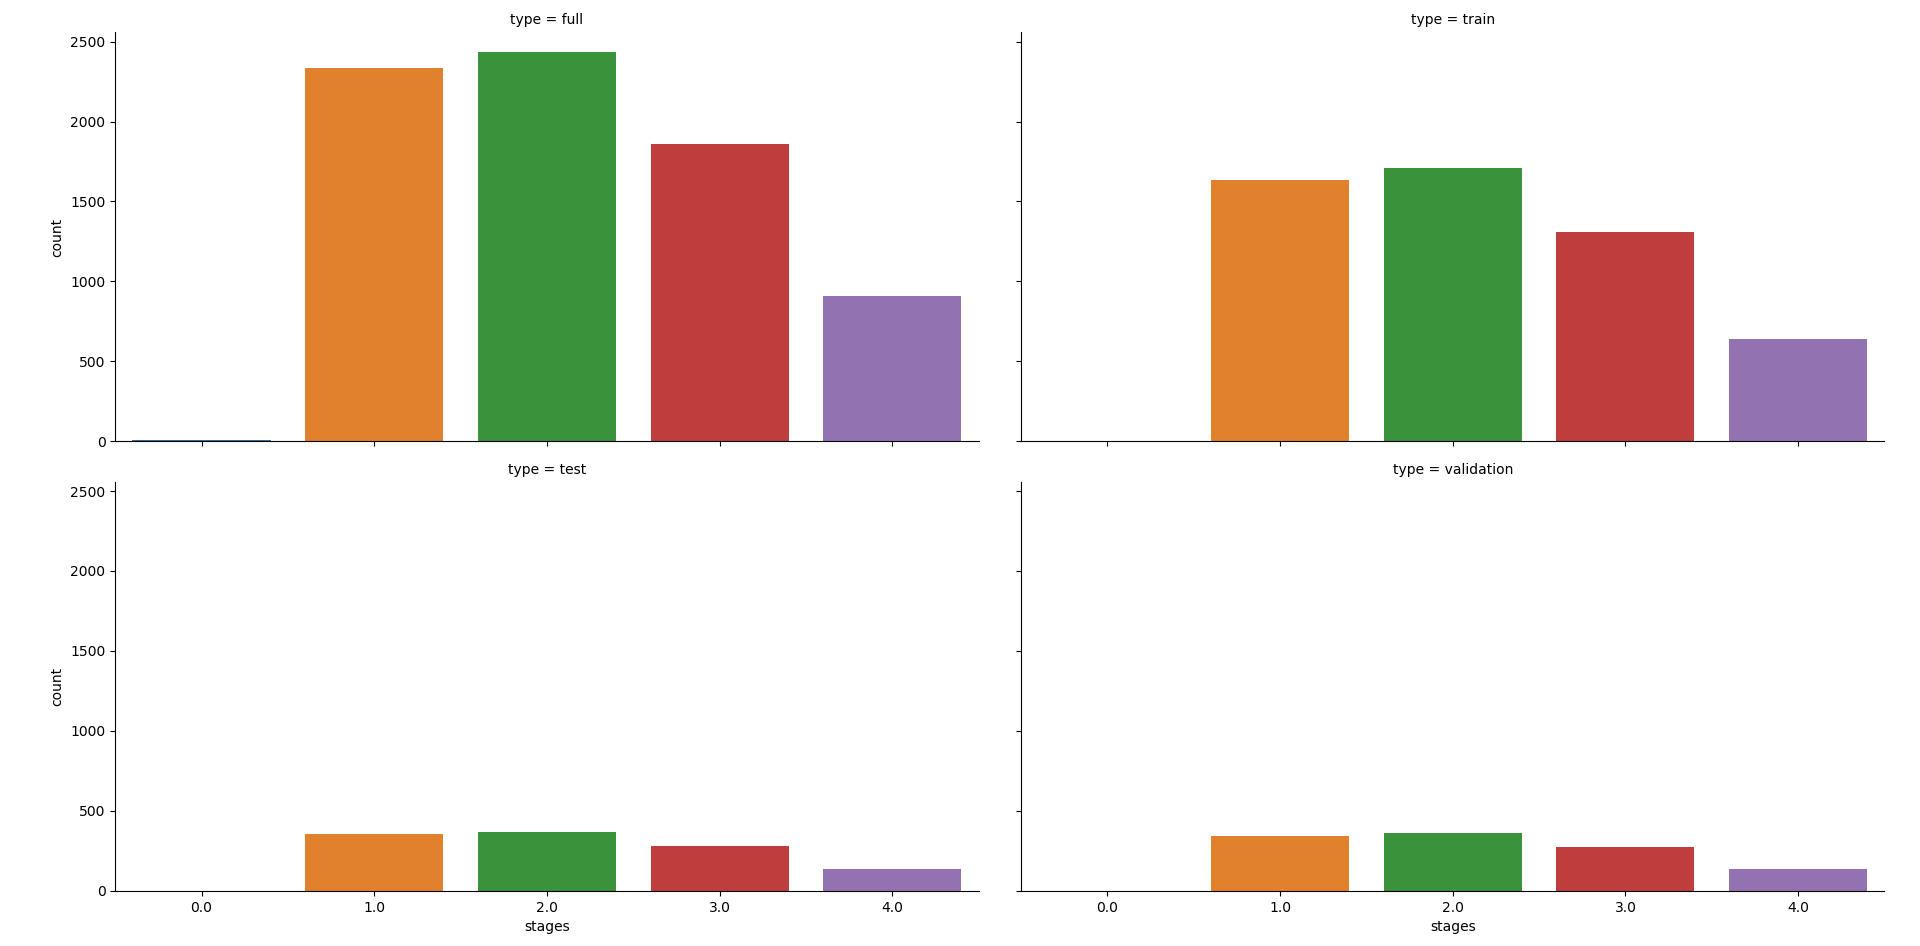
\includegraphics[width=\linewidth]{images/split_stages.png}   
    \caption[Splitting - stages]{Splitting of the main dataset to train, validation and test set with respect to stages}
    \label{fig:split_stages}
\end{figure}

\begin{figure}
    \centering
    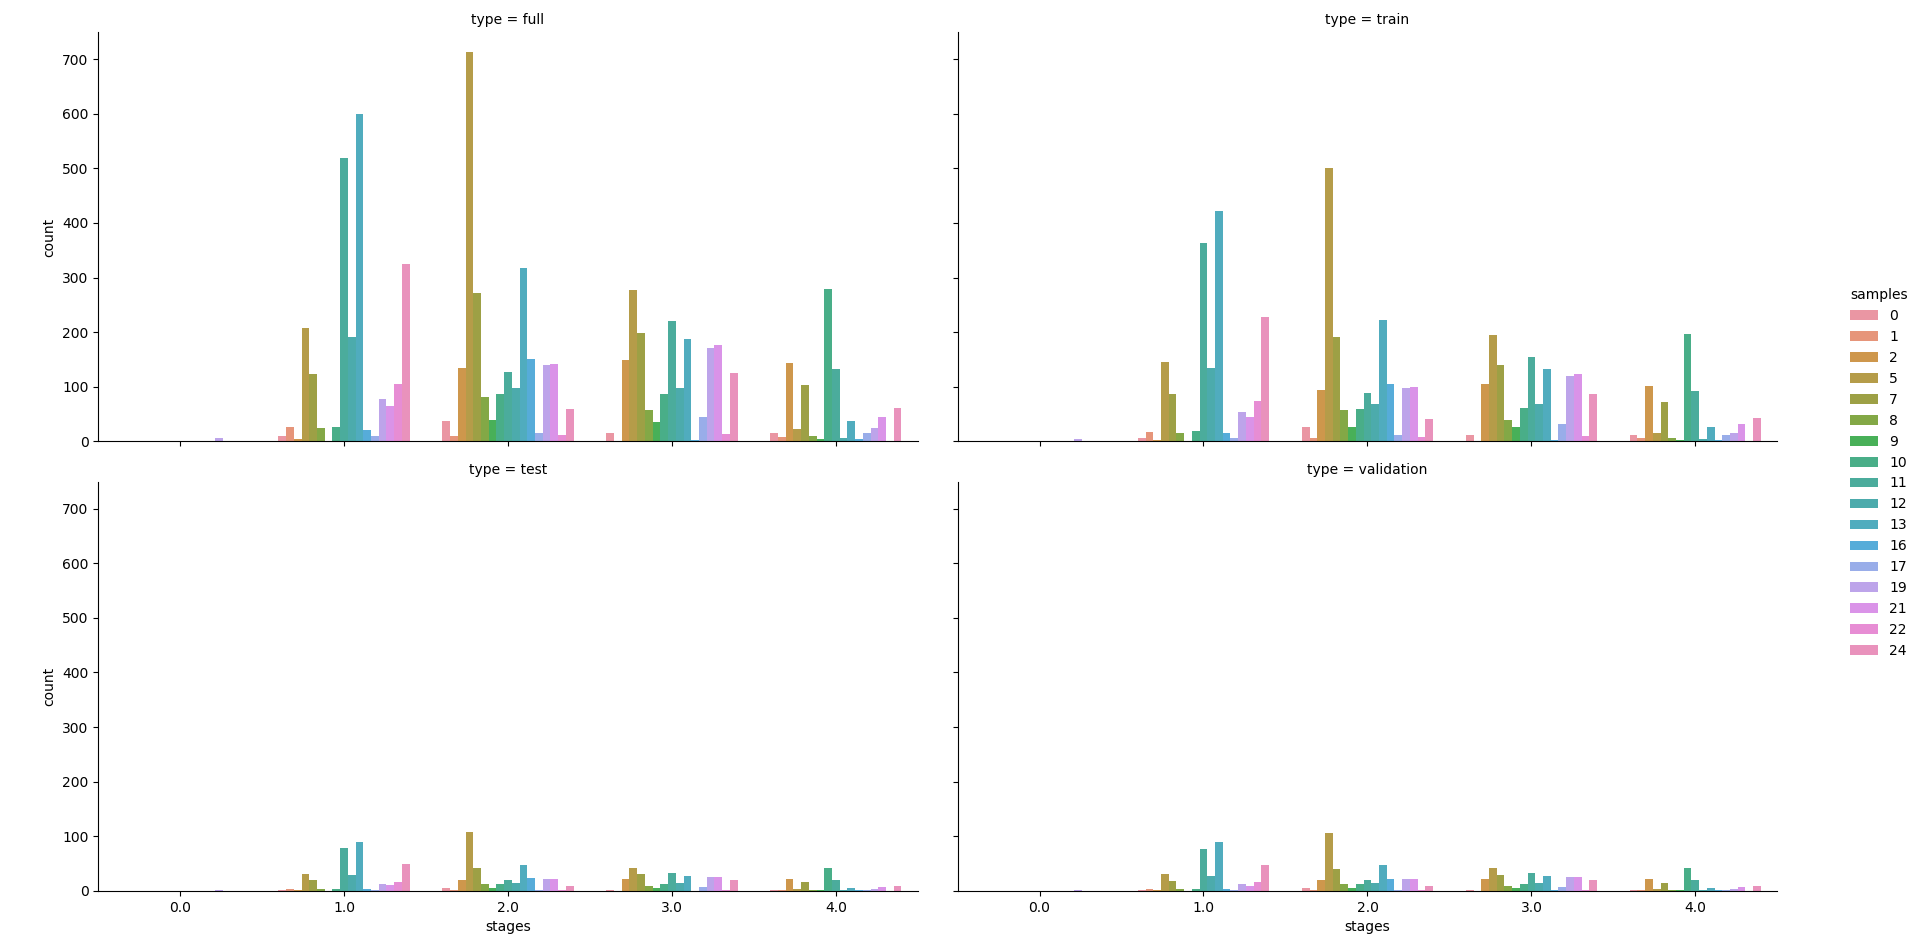
\includegraphics[width=\linewidth]{images/split_all.png}
    \caption[Splitting - combined]{Splitting of the main dataset to train, validation and test set with respect to tissue type and stages}
    \label{fig:split_all}
\end{figure}

\newpage
\section{Neural networks}
The main goal of this work was to build neural networks for classification based on the cancer expression data.
In this section, we will present the architecture of the neural networks used.

\subsection{PyTorch library}
For building neural networks, we used the python library PyTorch.
The PyTorch library is primarily developed by Facebook's artificial intelligence research group. \cite{pytorch}
In comparison with other AI frameworks, PyTorch belongs to one of the most popular with wide support for the scientific community.
It is a lower-level API focused on work with array expression which directly encourages the understanding of deep learning concepts.
Its lower-level approach ensures that the programmer has more control over the architecture.
Despite its lower-level approach, it provides many methods usually used in artificial intelligence designs like automatic differentiation and backpropagation.

\subsection{Dataset object}
PyTorch provides an option to define custom datasets.
This option is an excellent way to provide the data for training of the neural network because it makes the code cleaner and more intuitive.
It also enables to train the model on shuffled batches.
The shuffled batches can make the process of training more stable and less likely to jump over optimal values of parameters.
In our project, we made use of these benefits by using the abstract \verb'Dataset' class and created custom class \verb'MyDataset' extending the \verb'Dataset' class.

\subsection{Feed forward neural network}
We defined our neural network class in such a way that the number of layers and units inside those layers could be passed to the model as a parameter.
This parameter was in the format of the list of integers separated by \verb'-' separator.
In this format, the first integer represented the size of the input layer, the last integers represented the size of the output layer, and every integer in between represented the sizes of the hidden layers.
This flexible architecture allowed us to train models with many different parameters using one piece of software.
We created this architecture using PyTorch object \verb'ModuleList' to which we added Linear layers with required parameters.
For each hidden layer, we used ReLU nonlinearity function, and for the output layer, we used the softmax function.

\begin{figure}
    \centering
    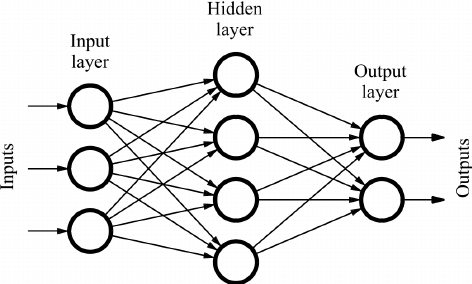
\includegraphics[width=0.7\linewidth]{images/ff_nn.png}
    \caption[Neural network - example]{Neural network architecture which could be generated using the \texttt{3-4-2} expression as a parameter}
    \label{fig:ff_nn}
\end{figure}

\subsection{Pathways neural network}
In the pathways neural network architecture, we wanted to incorporate additional information about the genes into the neural network.
For this, we used KEGG data mentioned in Subsection \ref{subsec:kegg}.
The architecture consisted of our custom layer named Pathways followed by Linear layers similar to the feedforward neural networks.
The Pathways layer represented the membership of a gene to a particular biochemical pathway assigned to the gene in the KEGG database.
For this purpose, we used the binary matrix where rows represented genes and columns designated pathways.
The Pathways layer then performed entrywise matrix multiplication between binary matrix and weights.
This multiplication effectively sets the majority of the connections to zero with the remaining connections representing the membership of the gene to a pathway.
The product was then used for transition between the input layer to the first hidden layer.

\subsection{Training and regularization of the neural networks}
During the training, we loaded training observations to our custom dataset class.
This class was then passed to the built-in \verb'DataLoader' class, which allowed us to train in shuffled batches.
We also programmed the training procedure to be able to use a graphical processing unit (GPU) for higher speed.
As an optimizer, we used \verb'Adam' - adaptive moment estimation optimizer \cite{kingma2014adam} with \verb'BCEWithLogitsLoss' loss function. 
After each run through the whole training dataset (epoch), we recorded the training loss, training accuracy, validation loss and validation accuracy.
We also stored a pickled python object of the model after each epoch.
The idea here was to perform a form of regularization called early stopping, where we would choose the model with the lowest validation error.
Together with this regularization, we also used dropout regularization \cite{srivastava2014dropout}.
The dropout regularization temporarily removes some of the neurons and all of their incoming and outgoing connections during the training of the model. 
This procedure is a good approximation for averaging over exponentially many models.

Furthermore, we tried L2 regularization, which reduces the magnitude of the trained parameters. 
This regularization needs a hyperparameter for the strength of reduction. 
To estimate this hyperparameter, we ran through multiple options.
The validation error using different levels of the L2 hyperparameter were visualized in Figure \ref{fig:L2_reg}.

\begin{figure}
    \centering
    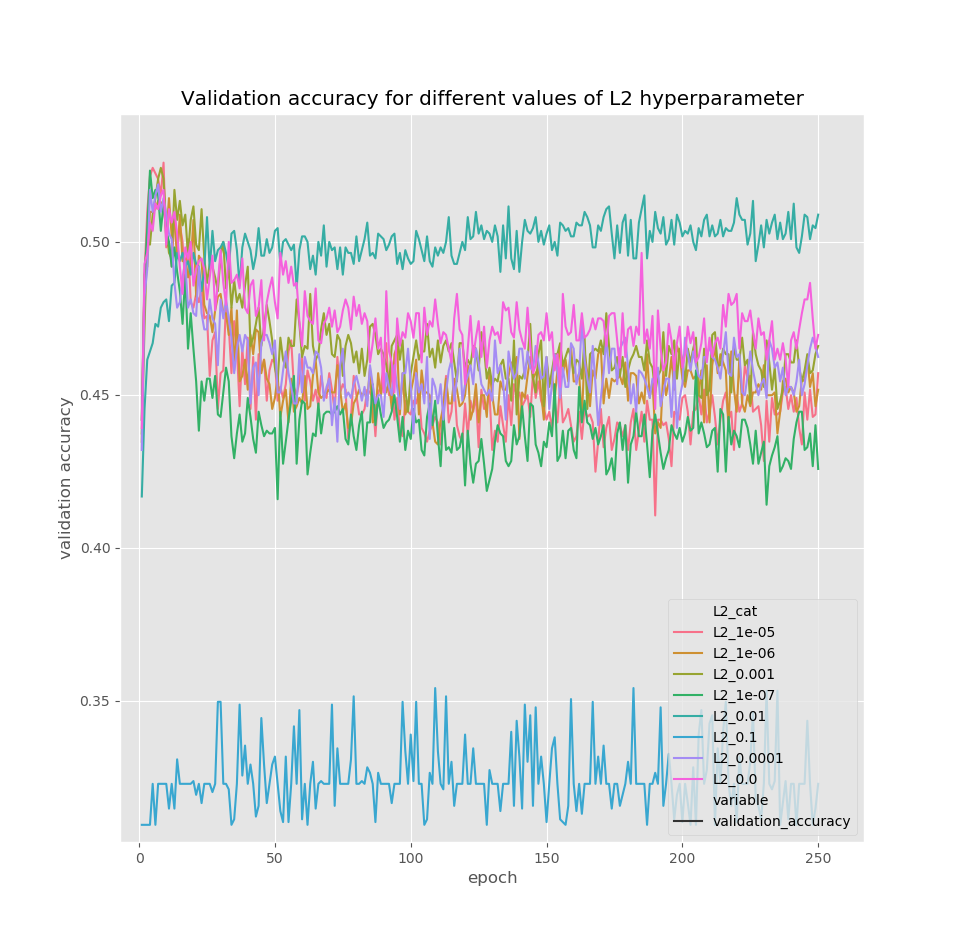
\includegraphics[width=0.7\linewidth]{images/val_acc_v2.png}
    \caption[L2 choice]{Validation accuracy across the epochs with different choice of L2 hyperparameter.}
    \label{fig:L2_reg}
\end{figure}